\section{Experimentación y Conclusiones}

Para un nuevo conjunto de instancias, generado de la misma manera que el que usamos para elegir la mejor configuración, corrimos los tests de tiempos de ejecución y de calidad y comparamos con la primera tanda de instancias.

\subsection{Comparación de tiempos de ejecución}

Esperábamos que esto no se vea afectado por el nuevo conjunto de instancias, que es lo que efectivamente ocurre. Por claridad, separamos los gráficos por profundidad:

\begin{figure}[H]
    \begin{minipage}[t]{\linewidth}
		\centering
		\frame{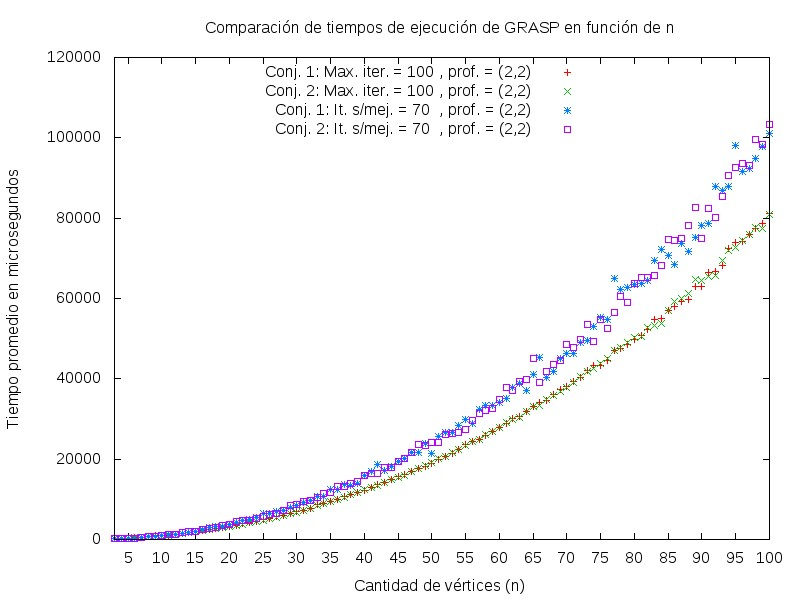
\includegraphics[width=\textwidth]{ejercicio-6-comparacion-tiempos-grasp-(2,2).jpg}}
		\label{fig:ejercicio-6-tiempos-grasp-2-2}
    \end{minipage}
\end{figure}

\begin{figure}[H]
    \begin{minipage}[t]{\linewidth}
		\centering
		\frame{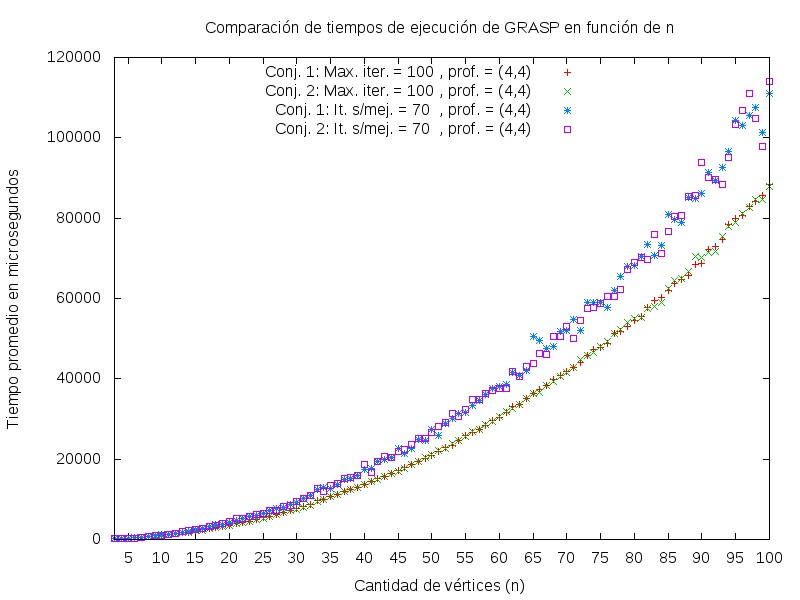
\includegraphics[width=\textwidth]{ejercicio-6-comparacion-tiempos-grasp-(4,4).jpg}}
		\label{fig:ejercicio-6-tiempos-grasp-4-4}
    \end{minipage}
\end{figure}

\subsection{Comparación de calidades}

Este test sí puede dar lugar a diferencias apreciables, ya que fijamos una configuración que no tenemos garantía de que sea óptima. Veamos primero la forma que tienen las calidades solamente del segundo conjunto:

\begin{figure}[H]
    \begin{minipage}[t]{\linewidth}
		\centering
		\frame{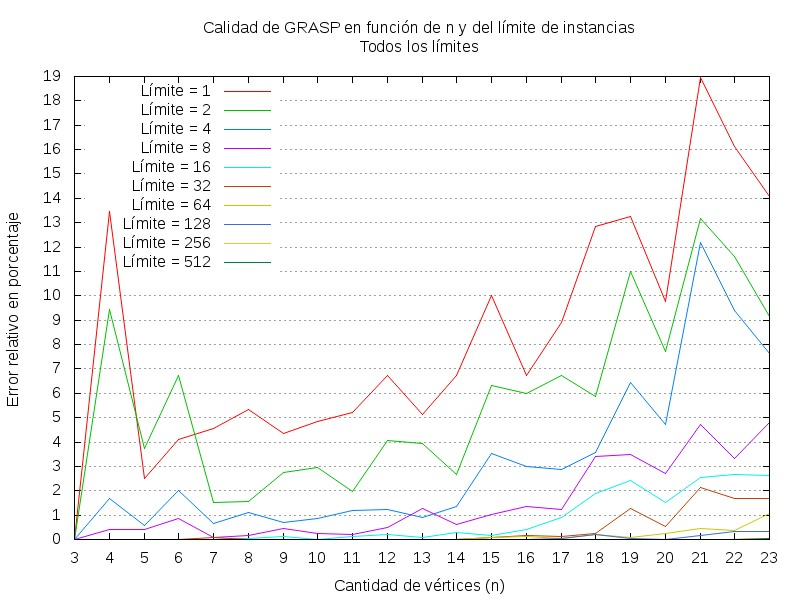
\includegraphics[width=\textwidth]{ejercicio-5-calidad-todos-conjunto-2.jpg}}
		\label{fig:ejercicio-6-calidad-todos-conjunto-2}
        \caption{Calidad del segundo conjunto de instancias}
    \end{minipage}
\end{figure}

A simple vista parece ser similar al gráfico obtenido para el primer conjunto, con los errores relativos creciendo con el $n$. Hagamos una comparación de las calidades de los mejores límites de iteraciones de un conjunto, contra el nuevo:

\begin{figure}[H]
	\begin{minipage}[t]{0.5\linewidth}
		\centering
		\frame{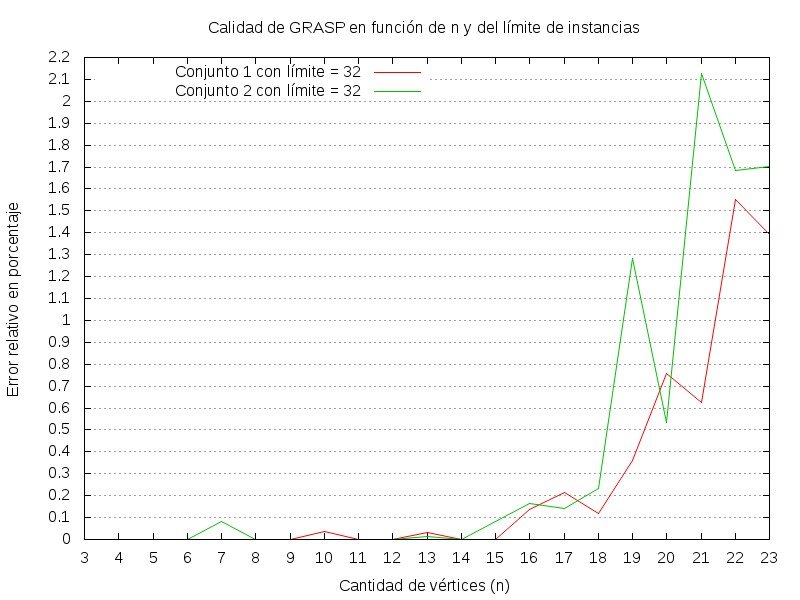
\includegraphics[width=\textwidth]{ejercicio-6-calidad-comparacion-n-32.jpg}}
		\caption{Comparación de calidad para límite de iteraciones $=$ 32}
		\label{fig:ejercicio-6-calidad-comparacion-n-32}
	\end{minipage}
	\begin{minipage}[t]{0.5\linewidth}
		\centering
		\frame{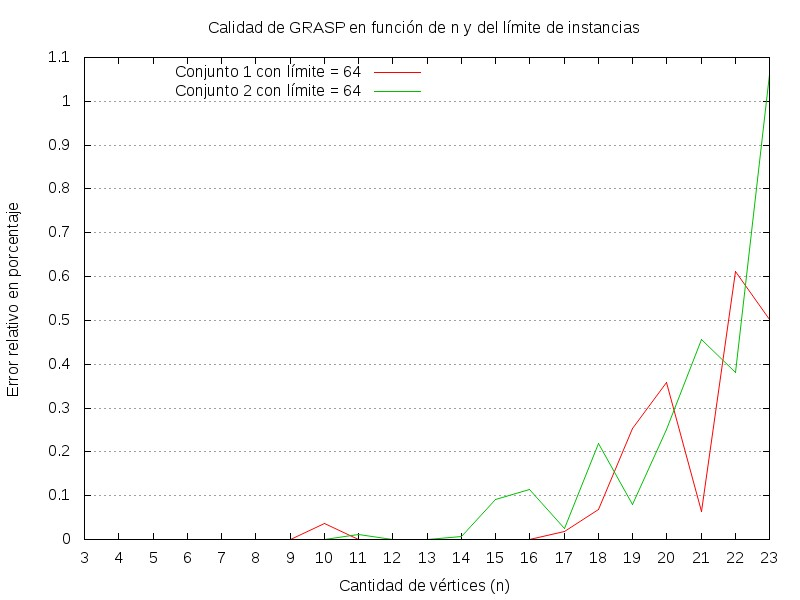
\includegraphics[width=\textwidth]{ejercicio-6-calidad-comparacion-n-64.jpg}}
		\caption{Comparación de calidad para límite de iteraciones $=$ 64}
		\label{fig:ejercicio-6-calidad-comparacion-n-64}
	\end{minipage}
\end{figure}

Para 32 iteraciones, el nuevo conjunto de instancias devuelve soluciones con una calidad peor para la mayoría de los casos, llegando a tener en los peores casos el doble de error relativo que el primer conjunto. Para 64, es menos claro, aunque para 14 y 15 nodos ni siquiera se llega a una solución óptima en el segundo conjunto pero sí en el primero, y para $n = 23$ se duplica el error relativo con respecto al primer conjunto.

\begin{figure}[H]
	\begin{minipage}[t]{0.5\linewidth}
		\centering
		\frame{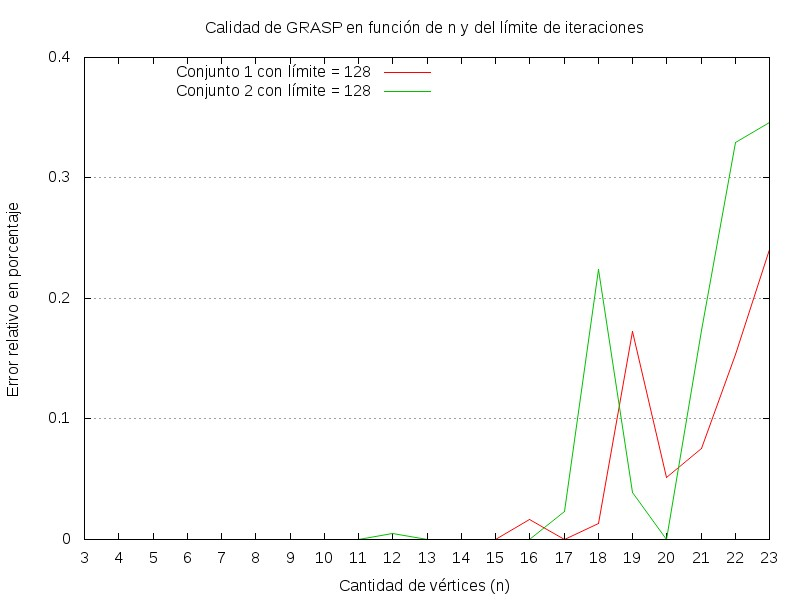
\includegraphics[width=\textwidth]{ejercicio-6-calidad-comparacion-n-128.jpg}}
		\caption{Comparación de calidad para límite de iteraciones $=$ 128}
		\label{fig:ejercicio-6-calidad-comparacion-n-128}
	\end{minipage}
	\begin{minipage}[t]{0.5\linewidth}
		\centering
		\frame{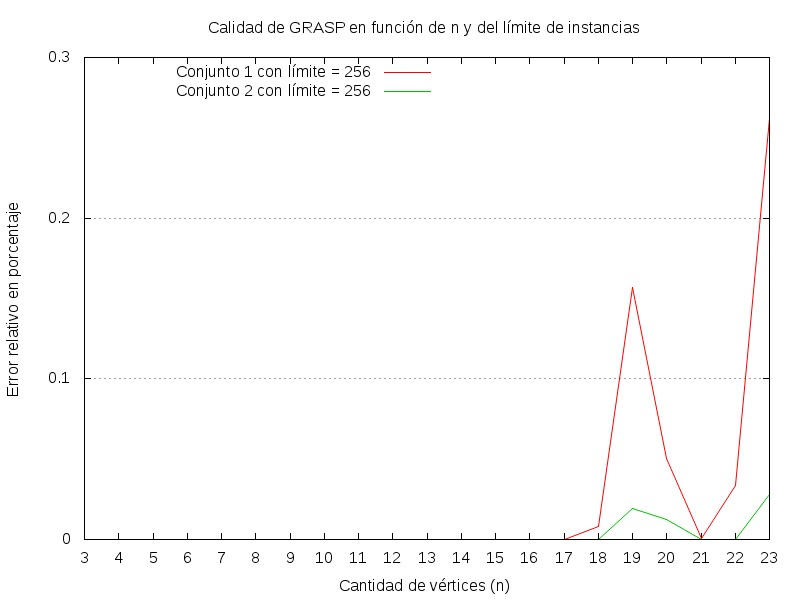
\includegraphics[width=\textwidth]{ejercicio-6-calidad-comparacion-n-256.jpg}}
		\caption{Comparación de calidad para límite de iteraciones $=$ 256}
		\label{fig:ejercicio-6-calidad-comparacion-n-256}
	\end{minipage}
\end{figure}

Para el límite de 128 iteraciones ocurre algo similar que para 64, aunque para 256 el que obtiene claramente la peor calidad es el primer conjunto, mientras el segundo se mantiene incluso por debajo de la barrera de $0.05\%$.

\subsection{Conclusiones}

Discutimos sobre criterios de parada y sobre la selección de candidatos de la golosa aleatorizada, y elegimos una configuración en base a los resultados obtenidos para un primer conjunto de instancias.

Testeamos sobre dos criterios de parada y comentamos sus beneficios y problemas. En una aplicación real, sería conveniente por lo menos usar una combinación de ambos criterios, es decir, iteraciones sin mejora pero con un límite máximo de iteraciones global. Por otro lado, para distintos valores de $n$, vimos que es conveniente variar los límites para reducir el tiempo de ejecución, por lo cual sería interesante tener límites dinámicos según la cantidad de vértices del grafo de entrada.

Para la selección de candidatos de la golosa aleatorizada, testeamos varios niveles de profundidad de elección de vértice y de elección de conjunto. No fue claro en particular que la mejor profundidad sea $(4,4)$, ya que aunque resultó ganadora, los errores relativos eran tan cercanos a cero que bien podría tratarse de una acumulación de los errores de cálculo inherentes a la aritmética finita. Sí es más claro que es más importante aleatorizar la elección del conjunto destino.

Elegimos la configuración de iteraciones sin mejora y profundidad de elección de vértice-conjunto $(4,4)$ y comparamos los resultados del primer conjunto con un nuevo conjunto de iteraciones. Vimos que aunque los tiempos de ejecución se mantuvieron intactos, la calidad no fue la esperada, teniendo en algunos casos el doble de error relativo para el segundo conjunto. Esto sugiere que no hay garantía de que una configuración funcione relativamente bien siempre, la única garantía de calidad parece ser la cantidad de iteraciones que realiza la GRASP.
